\documentclass[slovene,11pt,a4paper]{article}
\usepackage[margin=2cm,bottom=2cm,foot=1.5cm]{geometry}
% \documentclass[slovene,11pt,a4paper]{article}
% \usepackage[margin=1.7cm,bottom=3cm,foot=1.5cm]{geometry}
\setlength{\parindent}{0pt}
\setlength{\parskip}{0.5ex}

\usepackage[pdftex]{graphicx}
\usepackage{pgffor}
\usepackage{subcaption}
% \usepackage{a4wide} %najaci package
\usepackage[utf8]{inputenc}
\usepackage[slovene]{babel}
\usepackage{color}
\usepackage{graphicx}
% \usepackage{subfigure}
\usepackage{imakeidx}
\usepackage{adjustbox}
\usepackage{float}
\usepackage{amsmath}
\usepackage{mathtools}
\usepackage{tikz}
\usepackage{amssymb}
\usepackage{listings}
\usepackage{siunitx}
\usepackage{hyperref}
\usepackage{amsfonts}
\usepackage{mathrsfs}
\def\phi{\varphi}
\def\eps{\varepsilon}
\def\theta{\vartheta}

\newcommand{\thisyear}{2024/25}

\renewcommand{\Re}{\mathop{\rm Re}\nolimits}
\renewcommand{\Im}{\mathop{\rm Im}\nolimits}
\newcommand{\Tr}{\mathop{\rm Tr}\nolimits}
\newcommand{\diag}{\mathop{\rm diag}\nolimits}
\newcommand{\dd}{\,\mathrm{d}}
\newcommand{\ddd}{\mathrm{d}}
\newcommand{\ii}{\mathrm{i}}
\newcommand{\lag}{\mathcal{a}\!}
\newcommand{\ham}{\mathcal{H}\!}
\newcommand{\four}[1]{\mathcal{F}\!\left(#1\right)}
\newcommand{\bigO}[1]{\mathcal{O}\!\left(#1\right)}
\newcommand{\sh}{\mathop{\rm sinh}\nolimits}
\newcommand{\ch}{\mathop{\rm cosh}\nolimits}
\renewcommand{\th}{\mathop{\rm tanh}\nolimits}
\newcommand{\erf}{\mathop{\rm erf}\nolimits}
\newcommand{\erfc}{\mathop{\rm erfc}\nolimits}
\newcommand{\sinc}{\mathop{\rm sinc}\nolimits}
\newcommand{\rect}{\mathop{\rm rect}\nolimits}
\newcommand{\ee}[1]{\cdot 10^{#1}}
\newcommand{\inv}[1]{\left(#1\right)^{-1}}
\newcommand{\invf}[1]{\frac{1}{#1}}
\newcommand{\sqr}[1]{\left(#1\right)^2}
\newcommand{\half}{\frac{1}{2}}
\newcommand{\thalf}{\tfrac{1}{2}}
\newcommand{\pd}{\partial}
\newcommand{\Dd}[3][{}]{\frac{\ddd^{#1} #2}{\ddd #3^{#1}}}
\newcommand{\Pd}[3][{}]{\frac{\pd^{#1} #2}{\pd #3^{#1}}}
\newcommand{\avg}[1]{\left\langle#1\right\rangle}
\newcommand{\norm}[1]{\left\Vert #1 \right\Vert}
\newcommand{\braket}[2]{\left\langle #1 \vert#2 \right\rangle}
\newcommand{\obraket}[3]{\left\langle #1 \vert #2 \vert #3 \right \rangle}
\newcommand{\hex}[1]{\texttt{0x#1}}

\renewcommand{\iint}{\mathop{\int\mkern-13mu\int}}
\renewcommand{\iiint}{\mathop{\int\mkern-13mu\int\mkern-13mu\int}}
\newcommand{\oiint}{\mathop{{\int\mkern-15mu\int}\mkern-21mu\raisebox{0.3ex}{$\bigcirc$}}}

\newcommand{\wunderbrace}[2]{\vphantom{#1}\smash{\underbrace{#1}_{#2}}}

\renewcommand{\vec}[1]{\overset{\smash{\hbox{\raise -0.42ex\hbox{$\scriptscriptstyle\rightharpoonup$}}}}{#1}}
\newcommand{\bec}[1]{\mathbf{#1}}


\newcommand{\bi}[1]{\hbox{\boldmath{$#1$}}}
\newcommand{\bm}[1]{\hbox{\underline{$#1$}}}

\title{
\sc\large Matematično-fizikalni praktikum \thisyear \\
\bigskip
\bf\Large 8.~naloga: Robni problem lastnih vrednosti
}
\author{Tadej Tomažič}
\date{}

\makeindex[columns=3, title=Alphabetical Index, intoc]

\begin{document}


\pagenumbering{gobble} 
\author{Tadej Tomažič}
\date{\today}

\maketitle

\newpage
\pagenumbering{arabic}
\tableofcontents
\listoffigures
\newpage
\vspace{-1cm}
\section{Navodilo}

Za reševanje začetnih problemov s parcialnimi diferencialnimi
enačbami (PDE) imamo na voljo dva obsežna razreda metod.
Pri {\sl diferenčnih metodah\/} na neki način aproksimiramo
časovne in krajevne parcialne odvode s končnimi diferencami.
Reševanje PDE nato prevedemo na reševanje algebrajskih enačb
ali sistemov enačb za približne vrednosti funkcij, ki v teh
diferencah nastopajo.  Diferenčne metode spoznamo pri
naslednji vaji.  Pri tej vaji obravnavamno {\sl spektralne metode\/}:
pri njih iskano rešitev formalno izrazimo z nekim naborom funkcij,
nato pa v času spremljamo koeficiente v takem razvoju.  Kako se
selimo med krajevno in časovno sliko problema, je odvisno
od posamezne metode.  Osnovne prijeme spoznamo ob Fourierovi
metodi in  metodi končnih elementov s kubičnimi $B$-zlepki ($B$-splines).

Fizikalno ozadje naj bo enorazsežna difuzijska enačba,
ki opisuje na primer temperaturno polje $T(x,t)$ v homogeni
neskončni plasti s končno debelino $a$ brez izvorov toplote:
\begin{equation*}
\Pd{T}{t} = D\Pd[2]{T}{x}
 \>, \qquad 0\le x \le a \>, \qquad D={\lambda\over \rho c} \>.
\end{equation*}
Temperaturo v poljubni točki $x$ ob času $t$ izrazimo
s Fourierovo vrsto
\begin{equation*}
T(x,t) \simeq \sum_{k=0}^{N-1} \widetilde{T}_k(t)
e^{-2\pi\mathrm{i} f_k x} \>,
\end{equation*}
kjer je $f_k = k/a$, torej
\begin{equation*}
\sum_k {\partial\widetilde{T}_k(t)\over\partial t}\,
\mathrm{e}^{-2\pi\mathrm{i} f_k x} =
D \sum_k (-4\pi^2 f_k^2) \, \widetilde{T}_k(t) \,
\mathrm{e}^{-2\pi\mathrm{i} f_k x} \>.
\end{equation*}
Od tod sledi evolucijska enačba za Fourierove koeficiente
\begin{equation}
{\partial\widetilde{T}_k(t)\over\partial t} =
D \, (-4\pi^2 f_k^2) \, \widetilde{T}_k(t) \>.
\label{eq:num}
\end{equation}
Pogosto uporabimo spektralno reprezentacijo za krajevni odvod,
medtem ko časovni korak naredimo z neko eksplicitno integracijsko
shemo, na primer kar po Eulerju
\begin{equation}
\widetilde{T}_k(t+h) = \widetilde{T}_k(t)
+ h D (-4\pi^2 f_k^2) \widetilde{T}_k(t) \>.
\label{ffteuler}
\end{equation}
Reprezentacijo $T(x,t)$ v običajnem prostoru nato dobimo
z obratno Fourierovo transformacijo.

\bigskip

Tu lahko v splošnem časovni korak izvedeš po Eulerju, v tem konkretnem primeru
pa obstaja tudi enostavna analitična rešitev enačbe \ref{eq:num}, ki jo lahko uporabiš za primerjavo.
V numerični metodi tako najprej izračunaj Fourierovo reprezentacijo $\widetilde{T}_k(0)$
začetnega pogoja, nato pa jo po Eulerju evolviraj v času.
Pri tem moraš paziti na stabilnost Eulerjeve diferenčne sheme:
pri katerem koli koraku mora veljati
\begin{equation*}
\left\vert \,
{\widetilde{T}_k(t+h)\over \widetilde{T}_k(t)} \,\right\vert
= \left\vert\, 1 + hD(-4\pi^2 f_k^2)\, \right\vert < 1 \>.
\end{equation*}

Nekaj pozornosti zahteva tudi diskretizacija: za vsak $k$
seveda velja  $-f_\mathrm{Nyquist} < f_k < f_\mathrm{Nyquist}$ in s tem povezan
mo\v zen pojav \emph{aliasinga} (Kaj je že to?). Ta pojav lahko \v studira\v s,
\v ce se spomni\v s, da obstaja analiti\v cna re\v sitev FT Gaussove funkcije (je spet Gaussova funkcija) - kaj se z le-to dogaja znotraj dovoljenega frekvenčnega intervala?
\v Ce izbereš veliko število točk, je seveda smiselno uporabiti kar algoritem FFT.
Temperaturni profil $T_j(t)\equiv T(x,t)$ ob poljubnem času
nato dobiš z inverzno FFT.

\bigskip

Pri razvoju $T(x,t)$ nismo omejeni
na trigonometrične funkcije.  Rešitev PDE na $0\le x\le a$
lahko aproksimiramo tudi z drugačno vrsto funkcij,
na primer kubičnimi $B$-zlepki,
\begin{equation}
T(x,t) = \sum_{k=-1}^{N+1} c_k(t) B_k(x) \>,
\label{Tcolloc}
\end{equation}
kjer je $B_k(x)$ kubični zlepek s središčem okrog $x=x_k$.
aastnosti $B$-zlepkov so navedene v dodatku.  Tako zasnujemo
{\sl metodo končnih elementov}, s \emph{kolokacijskim pogojem}, da naj se zlepek
ujema z rešitvijo v določenih izbranih točkah.  Podobno kot pri Fourierovi metodi
tudi pri tej metodi zahtevamo, da razvoj~(\ref{Tcolloc})
zadošča osnovni PDE in robnim pogojem.  Razvoj~(\ref{Tcolloc})
vstavimo v PDE in izvrednotimo rezultat pri $x=x_j$.
(Interval $[0,a]$ diskretiziramo na $N$ podintervalov širine
$\Delta x$ s točkami $x_j=j{\Delta x}$, kjer je $j=0,1,\ldots,N$.
Za kolokacijo je smiselno izbrati enake točke kot za diskretno
mrežo.)  Tako dobimo
$$
\sum_{k=-1}^{N+1} \dot{c}_k(t) B_k(x_j) =
D \sum_{k=-1}^{N+1} c_k(t) B_k''(x_j) \>, \quad j = 0,1,\ldots,N \>.
$$
Upoštevamo lastnosti $B$-zlepkov in dobimo sistem
diferencialnih enačb za koeficiente $c_j(t)$:
$$
\dot{c}_{j-1}(t) + 4\dot{c}_j(t) + \dot{c}_{j+1}(t)
= {6D\over{\Delta x}^2} \left(c_{j-1}(t) - 2c_j(t) + c_{j+1}(t) \right) \>,
$$
kjer je $j=0,1,\ldots,N$.  Iz robnega pogoja pri $x=0$
ugotovimo $c_{-1} = -4c_0 - c_1$. Če dodamo še zahtevo za 'naravni' kubični
zlepek, da je na robu $\sum_{k=-1}^{N+1} c_k(t) B_k''(x=(0,a))=0$, sledi
 $c_0=c_N=0$ in $c_{-1}=-c_1$ ter $c_{N-1}=-c_{N+1}$.
Reševanje enačbe~(\ref{Tcolloc}) smo torej prevedli
na reševanje matričnega sistema
$$
{\bi A}\frac{d\vec{c}}{dt} = {\bi B}\vec{c} \>,
$$
kjer je
$$
{\bi A} = \left(
\begin{array}{ccccccc}
4 & 1 \cr
1 & 4 & 1 \cr
  & 1 & 4 & 1 \cr
  &   &   & \vdots \cr
  &   &   & 1 & 4 & 1 & \cr
  &   &   &   & 1 & 4 & 1 \cr
  &   &   &   &   & 1 & 4
\end{array}
\right) \>, \qquad
{\bi B} = {6D\over{\Delta x}^2} \left(
\begin{array}{rrrrrrr}
-2 & 1 \cr
1 & -2 & 1 \cr
  & 1 & -2 & 1 \cr
  &   &   & \vdots \cr
  &   &   & 1 & -2 & 1 & \cr
  &   &   &   & 1 & -2 & 1 \cr
  &   &   &   &   & 1 & -2
\end{array}
\right)
$$
in $\vec{c} = (c_1(t), c_2(t), \ldots c_{N-1}(t))^\mathrm{T}$.
Začetni pogoj za PDE je $T(x_j,0) = f(x_j)$, torej je začetni
približek za kolokacijsko aproksimacijo
$$
{\bi A}\vec{c}^{\>0} = \vec{f} \>,
$$
kjer je $\vec{f}=(f(x_1),f(x_2),\ldots,f(x_{N-1}))^\mathrm{T}$.
To zdaj rešujemo s kako metodo, ki jo poznamo iz prejšnjih
nalog, recimo z eksplicitno Eulerjevo metodo: ob zaporednih
časih $n{\Delta t}$ dobimo
$$
\vec{c}^{\>n+1} = \vec{c}^{\>n} + {\Delta t}{ A}^{-1}{ B}\vec{c}^{\>n}
 = ( { 1} + {\Delta t}{ A}^{-1}{ B})\vec{c}^{\>n} \>.
$$
Ob poljubnem času nato dobimo temperaturni profil tako,
da znova izračunamo vsoto~(\ref{Tcolloc}).
Ker nam je že znano, da je Eulerjeva ob predolgih časovnih korakih
lahko nestabilna, lahko uporabimo stabilno implicitno metodo,
kjer v vsakem časovnem koraku rešujemo
$$
  \left( { A} - \frac{\Delta t}{2}{ B}\right)\vec{c}^{\>n+1} \>
 = \left( { A} + \frac{\Delta t}{2}{ B}\right)\vec{c}^{\>n} \>.
$$
\bigskip
{\sl Naloga:}
\begin{itemize}
  \item Reši difuzijsko enačbo v eni razsežnosti $x\in [0,a]$
z začetnim pogojem po plasti gaussovsko porazdeljene temperature
\begin{equation*}
  T(x,0) \propto \mathrm{e}^{-(x-a/2)^2 / \sigma^2}
\end{equation*}
(izberi razumne vrednosti za $D$, $a$ in $\sigma$)
in
\begin{enumerate}
 \item periodičnim robnim pogojem $T(0,t) = T(a,t)$.
 \item homogenim Dirichletovim robnim pogojem $T(0,t) = T(a,t)=0$.
\end{enumerate}
po Fourierovi metodi.
\item Kolokacijsko metodo uporabi ob Gaussovem začetnem pogoju
in homogenih Dirichletovih robnih pogojih $T(0,t)=T(a,t)=0$ ter primerjaj obe metodi.
\end{itemize}
{\sl Dodatna naloga:} Izberi si še kakšen primer začetnih pogojev,recimo:
$$
T(x,0) = f(x) = \sin (\pi x/a)
$$
 in preizkusi obe metodi.
\bigskip\bigskip

%\newpage

\hrule

\bigskip

\noindent {\bf Dodatek: kubični $B$-zlepki}

\bigskip

\noindent Kubični $B$-zlepki imajo obliko
$$
B_k(x) = \left\{
\begin{array}{ll}
  0
    & \quad\text{če~~} x \le x_{k-2} \cr
    & \cr
  \displaystyle\frac{1}{\Delta x^3} (x - x_{k-2})^3
    & \quad\text{če~~} x_{k-2} \le x \le x_{k-1} \cr
    & \cr
 +\displaystyle\frac{1}{\Delta x^3} (x - x_{k-2})^3
 -\displaystyle\frac{4}{\Delta x^3} (x - x_{k-1})^3
    & \quad\text{če~~} x_{k-1} \le x \le x_{k} \cr
    & \cr
    +\displaystyle\frac{1}{\Delta x^3} (x_{k+2} - x)^3
    -\displaystyle\frac{4}{\Delta x^3} (x_{k+1} - x)^3
    & \quad\text{če~~} x_{k} \le x \le x_{k+1} \cr
    & \cr
    \displaystyle\frac{1}{\Delta x^3} (x_{k+2} - x)^3
    & \quad\text{če~~} x_{k+1} \le x \le x_{k+2} \cr
    & \cr
  0
    & \quad\text{če~~} x_{k+2} \le x
\end{array}\right. \>
$$
\section{Rešitev}

Najprej si poglejmo avtokorelacijo za obe sovi.
\begin{figure}[h]
    \centering
    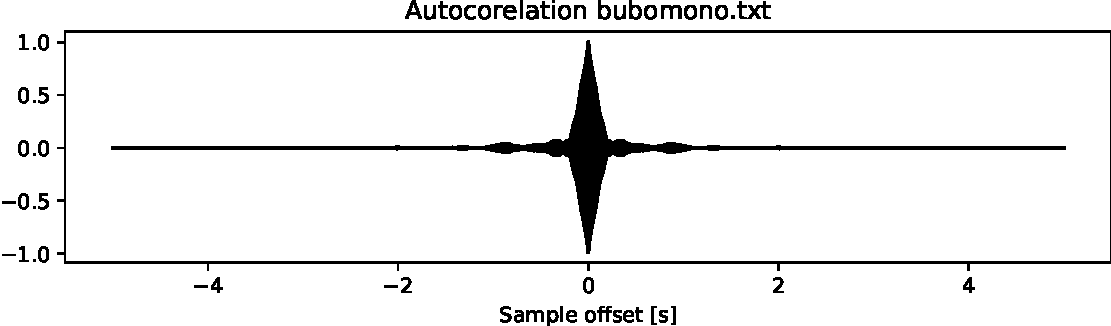
\includegraphics[width=12cm]{pdfs/bubomono.txt_acor.pdf}
    \vspace{10pt}
    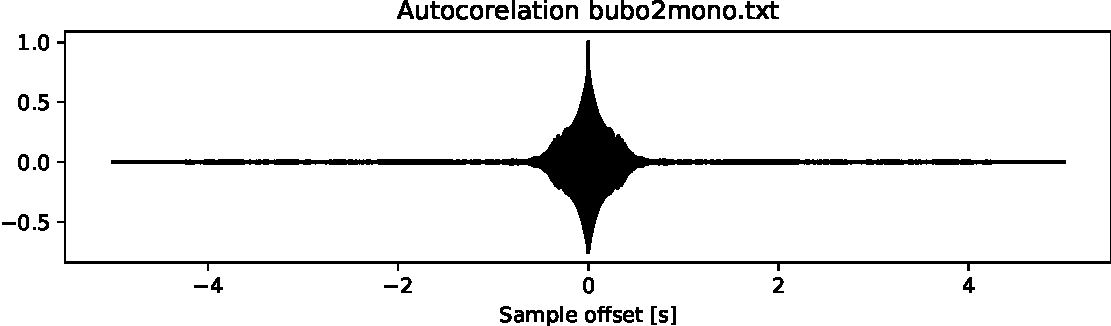
\includegraphics[width=12cm]{pdfs/bubo2mono.txt_acor.pdf}
    \caption{Avtokorelacija signala sov}
\end{figure}

Preden sem koreliral signal sem vektorja samplov normiral, tako da je
"najmočnejši" signal 1. To pomeni \[\|x\|_\infty = \max_i |x_i|\]

Poglejmo si še korelacije med sovami in posnetki:
\newpage
\begin{figure}[h]
    \centering
    \foreach \mix in {mix, mix1, mix2, mix22} {
        \foreach \sova in {bubomono, bubo2mono}{
            \includegraphics[width=8cm]{pdfs/cor_\mix.txt_\sova.txt.pdf}
        }
    }
    \caption{Korelacija sov in posnetkov iz narave}
\end{figure}
Tukaj je bila normalizacija drugače izbrana. Tukaj je bila narejena normalizacija korelacije. Če je varianca signala a $\sigma_a$,
potem je $ \mathbf{x} = \mathbf{x} / \left(\sigma_a \sigma_b |\mathbf{b}|\right)$. Sigma je izračunana z \verb|numpy.std()|.


Hitrosti so precej dolgčasno pričakovane ampak vseeno.
\begin{figure}[h]
    \centering
    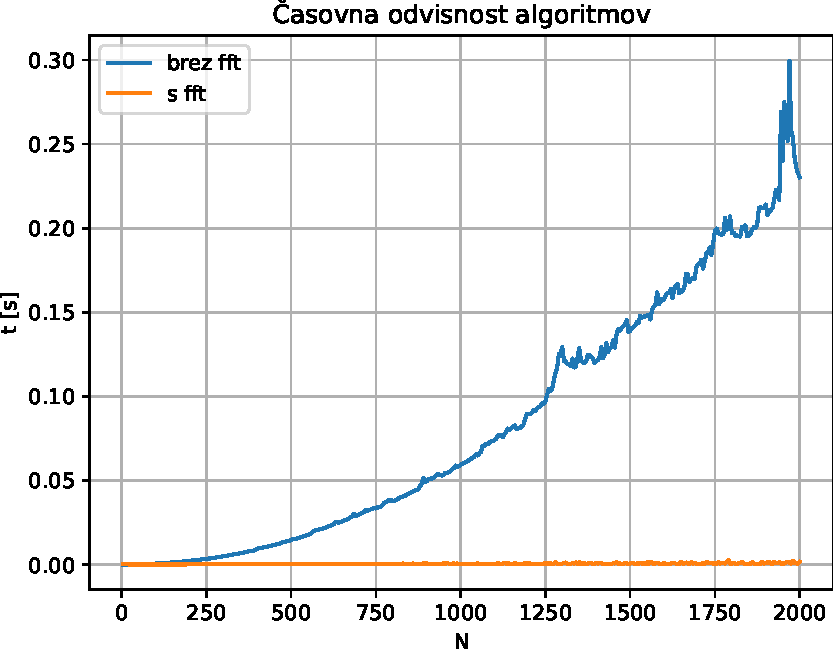
\includegraphics[width=8cm]{pdfs/cas-lin.pdf}
    \vspace{10pt}
    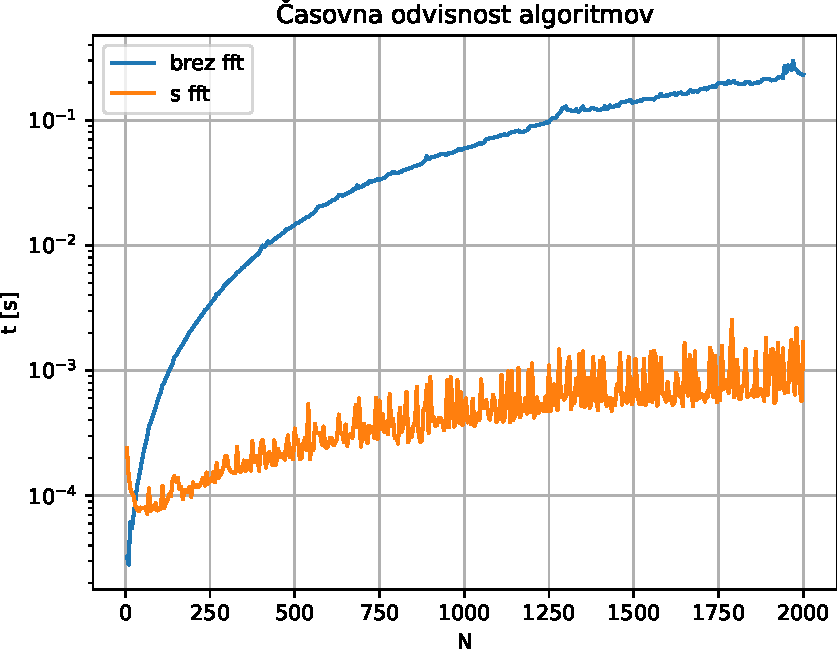
\includegraphics[width=8cm]{pdfs/cas-log.pdf}
    \caption{Hitrost algoritmov}
\end{figure}
\newpage
\section{Dodatna naloga}
Posnel sem dva človeka m in ž ko izgovarjata aaaaaaaaaaaa. Posnel sem jih tudi
ko bereta slovar. Gledal sem ali lahko spet zaznam ali gre za ž glas ali m glas.
Poglejmo si spektra njunega glasu.
\begin{figure}[h]
    \begin{center}
        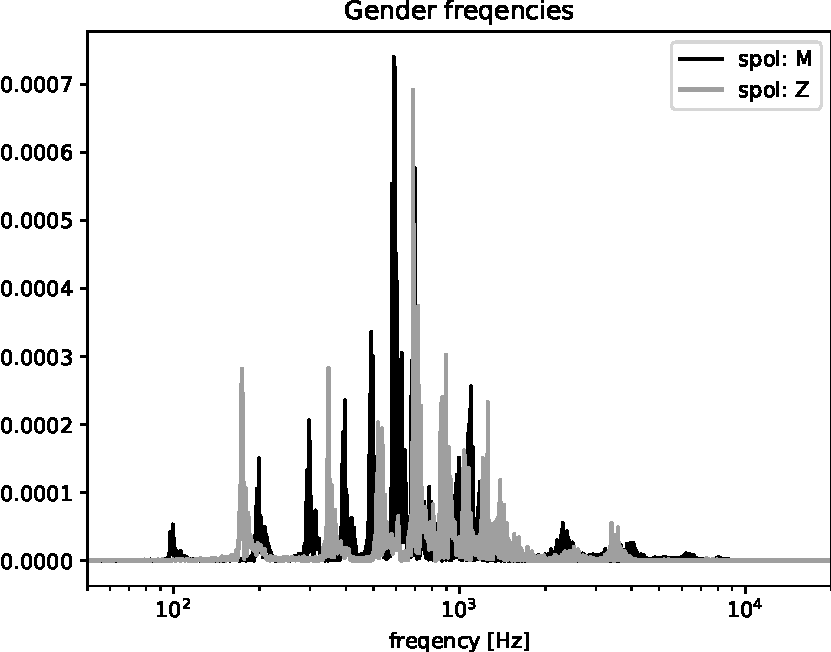
\includegraphics[width=12cm]{pdfs/fft_spol.pdf}
    \end{center}
    \caption{Barva glasu moškega in ženske}
\end{figure}

% Glasova sta bila prej normirana, saj je bil moški glas posnet bližje mikrofona.
% Poglejmo si zopet korelacijo med posnetki:
% \foreach \gender in {Z, M} {
%     \foreach \mix in {Glas\ 001, Glas\ 002}{
%         pdfs/cor_\gender_\mix.pdf 
%     }
% }
\begin{figure}[h]
    \begin{center}
        
    \foreach \gender in {Z, M} {%
        \foreach \mix in {001, 002} {%
            \includegraphics[width=8cm]{pdfs/cor_\gender_Glas\space\mix.pdf}%    
        }%
        \par
}%
    \end{center}
    
    \caption{Korelacija glasa človeka in posnetkov iz branja slovarja}
\end{figure}
\end{document}
